




\section{Competition}

	\subsection{Problem statement}
	Imagine you receive a letter in some PDF format. This letter has a title, a date, a sender and many other blocks. The project aims at, given a feature representation of a block, classifying the label(s) of this input blocks.




	\subsection{Data}
	\label{sec:dataset}

		In \fref{fig:FeatureExtraction1} you see a letter. For the Kaggle competition this letter has been analyzed and annotated with many blocks. Those blocks represent classes like, for example, a date, a page number or a name. All these blocks are our samples. The aim of the competition is to extract the common patterns of each classes to predict a new candidate. This task is called multi-label classification. 

		Below, we are first going to describe what are features corresponding to those boxes. Then we will describe the labels or the classes a box can belong to. And we will finish by describing the files also provided by the competition.		

		\begin{figure}[h]
			\begin{center}
				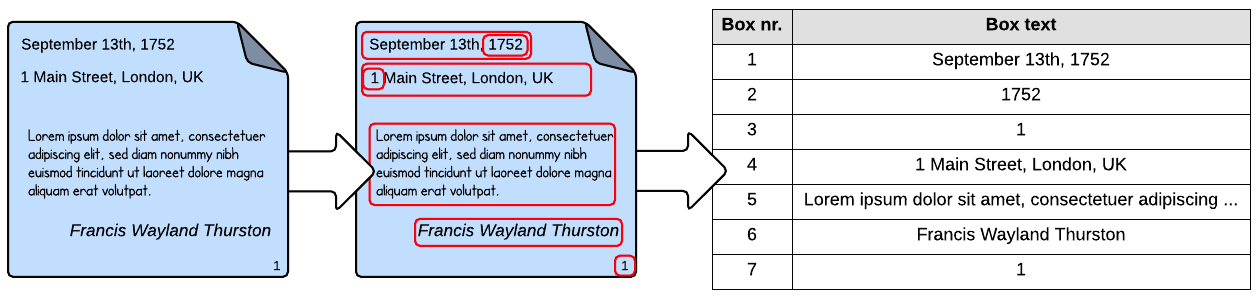
\includegraphics[width=0.9\textwidth]{FeatureExtraction1.png}
			\end{center}
			\caption{document segmentation from Kaggle website 
			\label{fig:FeatureExtraction1}}
		\end{figure}

		\subsubsection{features}
			A sample block is represented by 145 features. Those features include content feature, parsing feature, spatial feature and relational information features.

			\begin{itemize}
				\item The first feature we have is "Content feature". This feature is the direct representation of the text in a hashed format.
				\item The second feature is "Parsing feature". It indicates which kind of characters are present in the sample text. It can be for instance alphanumeric, numeric or text characters.
				\item Then come some "Spacial feature". This is about position and size of the block in the document.
			 	\item Finally, "Relational feature". They describe the hierarchies of the blocks. If a block has no parent, this value will be empty.
			\end{itemize}

			To these features can correspond either a value or nothing. If we have a value, it is either a real number, a discrete number, a boolean value or a text value. 


		\subsubsection{label}
			Any sample is related to a label or more. This is the aim of the project: labeling the samples. As mentioned previously a label could for instance be 'date' or 'pageNumber'. The competition provide 33 labels. Those labels are not explicit, we don't know what they correspond to.

			To a given sample is associated a 33d label vector with values 0 or 1. As there can be many labels, the vector size is not necessary 1. \fref{fig:labelcsv} shows an example of a sample labeling.


		\subsubsection{files}
			The data provided for this competition by Tradeshift consist of 3 csv files. 

			\begin{itemize}
				\item train.csv: File containing the training data. It has merely 1.7m lines of samples and 145 columns of features. Each cell has a either a real, a discrete, a boolean or a text value.
				\item trainLabels.csv: File containing label of data. It has a 3D array with merely 1.7m lines of samples, 33 columns of labels and each cell is either 0 or 1.
				\item test.csv: File containing the testing data. It has merely 0.4m lines of samples and 145 columns of features. Each cell has a either a real, a discrete, a boolean or a text value.
			\end{itemize}



	\subsection{evaluation}
		The work is evaluated by sending a csv file on the kaggle website. The csv file is then evaluated by the system.

		The csv file 'sampleSubmission.csv', is a 2 column csv file. On the first column is listed the sample number and a label and on the second column a prediction corresponding to this tuple {sample,label}.

		Once submitted, the file receive a score through a scoring function. The function scoring used is the negative logarithm of the likelihood, averaged over $N_t$ test samples and $K$ labels.
		Mathematically, this function is defined as follow:

		\begin{equation} \label{eq1}
			\begin{split}
				LogLoss & = \frac{1}{N_t \cdot K} \sum_{idx=1}^{N_t \cdot K} LogLoss_{idx} \\
				&= \frac{1}{N_t \cdot K} \sum_{idx=1}^{N_t \cdot K} [-y_{idx} \log{\hat{y}_{idx}} - (1-y_{idx}) \log{1-\hat{y}_{idx}}] \\
		        &= \frac{1}{N_t \cdot K} \sum_{i=1}^{N_t} \sum_{j=1}^{K} [-y_{ij} \log{\hat{y}_{ij}} - (1-y_{ij}) \log{1-\hat{y}_{ij}}]
			\end{split}
		\end{equation}

		This function gives an extreme punishment for wrong confident predictions. 

		For instance, the log-loss of one sample with one label predicting 0.001 instead of 1 (an extremely confident wrong prediction) is $-\log(0.001) = 3 $ whereas the log-loss of one sample with one label predicting 0.1 instead of 1 (a less confidently wrong prediction) is $\log(0.1) = 1$


